% SATE Meeting Note — Example (SLP team meeting, session R-S14)
% Same visual system as SATE-Therapy_Data_Tracking.tex — one family of documents.
% Compile with: pdflatex -output-directory=build SATE-Meeting_Note.tex (run twice)
% Overleaf: set the compiler to pdfLaTeX. \textls (microtype) does NOT work under XeLaTeX.
\documentclass[10pt,a4paper]{article}

% ---------- Fonts: serif body + sans headings/labels ----------
\usepackage[T1]{fontenc}
\usepackage[utf8]{inputenc}
\usepackage{mathpazo}
\usepackage[scaled=0.90]{helvet}
\usepackage{microtype}

% ---------- Layout (tight, single page) ----------
\usepackage[a4paper,top=0.8cm,bottom=0.85cm,left=1.4cm,right=1.4cm]{geometry}
\linespread{0.95}
\setlength{\parindent}{0pt}
\setlength{\parskip}{2pt}

% ---------- Color theme (shared SATE style) ----------
\usepackage[table,dvipsnames]{xcolor}
\definecolor{accent}{HTML}{215C68}
\definecolor{accentlt}{HTML}{9CC3CB}
\definecolor{goalgreen}{HTML}{2E7D4F}
\definecolor{amber}{HTML}{B8860B}
\definecolor{concern}{HTML}{B03A2E}
\definecolor{mono}{HTML}{6E6E6E}
\definecolor{fog}{HTML}{6E6E6E}

% ---------- Tables / lists ----------
\usepackage{booktabs}
\usepackage{tabularx}
\usepackage{array}
\usepackage{enumitem}
\renewcommand{\arraystretch}{1.15}

% ---------- Graphics / boxes ----------
\usepackage{tikz}
\usepackage[most]{tcolorbox}

% Section box: colored left border
\newtcolorbox{secbox}[1]{enhanced,colback=#1!5,colframe=#1!5,
  borderline west={2.5pt}{0pt}{#1},arc=1.5pt,
  left=6pt,right=6pt,top=3pt,bottom=3pt,boxsep=0pt,before skip=2.5pt,after skip=2pt}
% Note box: amber left border
\newtcolorbox{notebox}{enhanced,colback=amber!6,colframe=amber!6,
  borderline west={2.5pt}{0pt}{amber!80},arc=1.5pt,
  left=6pt,right=6pt,top=3pt,bottom=3pt,boxsep=0pt,before skip=3pt,after skip=3pt}

% ---------- Badges (rounded pills) ----------
\newcommand{\badge}[2]{\tcbox[on line,boxrule=0.4pt,arc=4pt,left=3pt,right=3pt,
  top=0.8pt,bottom=0.8pt,boxsep=0pt,colback=#1!13,colframe=#1!55!black!55]
  {\sffamily\scriptsize\bfseries\textcolor{#1!40!black}{#2}}}
\newcommand{\bEX}{\badge{mono}{EXAMPLE}}

% ---------- Small chips (timecodes, owners) ----------
\newcommand{\chip}[2]{\tcbox[on line,boxrule=0.4pt,arc=3.5pt,left=2.5pt,right=2.5pt,
  top=0.5pt,bottom=0.5pt,boxsep=0pt,colback=#1!12,colframe=#1!50!black!50]
  {\sffamily\fontsize{6}{6}\selectfont\bfseries\textcolor{#1!35!black}{#2}}}
\newcommand{\ts}[1]{\chip{accent}{#1}}      % timecode into the recording
\newcommand{\flagts}[1]{\chip{amber}{#1}}   % timecode the user marked with the flag button

% ---------- Section styling ----------
\usepackage{pifont}
\usepackage{titlesec}
\setcounter{secnumdepth}{0}
\titleformat{\section}[block]{\sffamily\bfseries\small}{}{0pt}
  {\textcolor{accent}{\rule[-2.5pt]{2.5pt}{10.5pt}}\hspace{0.55em}\color{accent}\textls[70]}
\titlespacing*{\section}{0pt}{0.5em}{0.2em}

% ---------- Info-bar field ----------
\newcommand{\infofield}[2]{{\sffamily\fontsize{5.5}{6.5}\selectfont\color{black!55}\textls[50]{#1}}\hspace{0.35em}{\small #2}}

% ---------- Bullet lists ----------
\newlist{pts}{itemize}{2}
\setlist[pts,1]{nosep,topsep=1.5pt,partopsep=0pt,parsep=1.5pt,itemsep=2.5pt,
  leftmargin=1.05em,label=\textcolor{accent}{\fontsize{4.5}{4.5}\selectfont\ding{108}}}
\setlist[pts,2]{nosep,topsep=2pt,partopsep=0pt,parsep=1pt,itemsep=1.5pt,
  leftmargin=1em,label=\textcolor{accent!45}{\fontsize{4.5}{4.5}\selectfont\ding{108}}}

\usepackage[hidelinks]{hyperref}
\pagestyle{empty}

\begin{document}

% ================= Header =================
\noindent
\begin{minipage}[b]{0.62\linewidth}
{\sffamily\LARGE\bfseries\color{accent} SATE - Meeting Note}\hspace{0.6em}\raisebox{2.5pt}{\bEX}
\end{minipage}\hfill
\begin{minipage}[b]{0.36\linewidth}\raggedleft
{\sffamily\scriptsize\color{black!65}Generated: 2026--09--03\quad Reviewed by: \rule[-1pt]{1.6cm}{0.3pt}\\[1pt]
Basis: meeting audio (SATE Record) $\cdot$ template \emph{Meeting}}
\end{minipage}
\\[2pt]
{\color{accentlt}\rule{\linewidth}{1pt}}

% ---------- Meeting subject: ONE child ----------
\vspace{2pt}
{\sffamily\large\bfseries\color{black!80}IEP progress review --- Child C}\hfill
{\sffamily\scriptsize\color{black!55}after session 6 of 8 $\cdot$ see \emph{SATE - Therapy Data Tracking}}

% ---------- Meeting info bar ----------
\vspace{2.5pt}
\begin{tcolorbox}[colback=gray!5,colframe=gray!25,boxrule=0.4pt,arc=2pt,
  left=6pt,right=6pt,top=2.5pt,bottom=2.5pt,boxsep=0pt]
\infofield{CHILD}{C}\quad
\infofield{AGE}{6;6}\quad
\infofield{RECORDING}{R-S14 $\cdot$ SATE-443EAC}\quad
\infofield{LENGTH}{26:12}\quad
\infofield{TEMPLATE}{Meeting}\\[2pt]
\infofield{PRESENT}{SLP $\cdot$ classroom teacher $\cdot$ parent $\cdot$ special-education coordinator}
\end{tcolorbox}

% ================= Timeline =================
\section{Recording Map \hspace{0.4em}{\normalfont\sffamily\scriptsize\color{black!55}(chapters detected from the transcript $\cdot$ \textcolor{amber!80!black}{\ding{116}} = flag button pressed during the meeting)}}

\vspace{1pt}
\noindent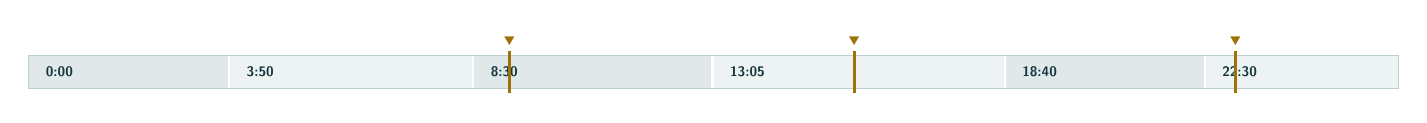
\begin{tikzpicture}[x=1cm,y=1cm]
  % chapter band: 0 s -> 17.4 cm covers the full 26:12
  % tint carried as a loop variable — never \ifnum inside a colour spec, and never \i as a
  % \foreach variable (\i is LaTeX's dotless i)
  \foreach \a/\b/\c in {0/2.55/14, 2.55/5.65/8, 5.65/8.69/14, 8.69/12.40/8, 12.40/14.94/14, 14.94/17.40/8}{
    \fill[accent!\c] (\a,0) rectangle (\b,0.42);}
  \foreach \x in {2.55, 5.65, 8.69, 12.40, 14.94}{
    \draw[white,line width=0.8pt] (\x,0) -- (\x,0.42);}
  \draw[accent!30,line width=0.4pt] (0,0) rectangle (17.40,0.42);
  % timecode inside each chapter
  \foreach \x/\t in {0.10/0:00, 2.65/3:50, 5.75/8:30, 8.79/13:05, 12.50/18:40, 15.04/22:30}{
    \node[anchor=west,font=\sffamily\fontsize{5.5}{5.5}\selectfont\bfseries,text=accent!60!black] at (\x,0.21) {\t};}
  % flag marks
  \foreach \x in {6.11, 10.49, 15.33}{
    \draw[amber!85!black,line width=1pt] (\x,-0.06) -- (\x,0.48);
    \node[font=\fontsize{4.5}{4.5}\selectfont,text=amber!85!black] at (\x,0.60) {\ding{116}};}
\end{tikzpicture}\\[1pt]
{\scriptsize\color{fog}\textbf{0:00} Progress since the last review \ $\cdot$\ \textbf{3:50} Goal 1 --- tense \& agreement \ $\cdot$\ \textbf{8:30} Goal 2 --- vocabulary \ $\cdot$\ \textbf{13:05} Goal 3 --- /s/ articulation \ $\cdot$\ \textbf{18:40} Home and classroom carryover \ $\cdot$\ \textbf{22:30} Service minutes and next steps}

% ================= Summary =================
\section{Summary}

\begin{secbox}{accent}
{\small The team reviewed C's progress after session 6 of 8. Two of the three goals are on trajectory for
their session-8 targets; initial /s/ at word level is the one behind, with the errors concentrated before
back vowels. The team agreed to keep service minutes unchanged and change what happens inside them,
rather than add time, and to re-decide at session 8.}
\end{secbox}

% ---------- Key points ----------
\section{Key Points}
{\footnotesize
\begin{pts}
\item \textbf{Goal 1 --- tense \& agreement:} 63\% independent this session against an 80\% target by
      session 8, up from 0\% at baseline; the team read the trajectory as on track.
  \begin{pts}
  \item Structured question frames pull higher than spontaneous narration (75\% vs.\ 50\%), so the
        frames stay in for now.
  \item All three misses were omissions, not overgeneralisations.
  \end{pts}
\item \textbf{Goal 2 --- vocabulary:} 8 of the 10 target words are now used spontaneously; two remain,
      and both are planned for session 7.
\item \textbf{Goal 3 --- initial /s/ is the goal behind trajectory:} 55\% at CVC word level against an
      80\% target, and the errors are not evenly spread.
  \begin{pts}
  \item Back-vowel words sit at 40\% against 70\% for front-vowel words --- consistent with the
        lateralised-/s/ profile in the baseline.
  \item Isolation has held above 90\% since session 5, so the level itself was not in question.
  \end{pts}
\item \textbf{In the classroom:} the teacher reports C now answers ``who is\,...'' questions in circle
      time without a model, but still rarely initiates.
\item \textbf{At home:} the parent reports the word list is being used during dressing and bath
      routines; \emph{sock} and \emph{hat} come spontaneously, \emph{button} is still imitated.
\end{pts}}

% ---------- Action items ----------
\section{Action Items \hspace{0.4em}{\normalfont\sffamily\scriptsize\color{black!55}(only a follow-up someone actually committed to or was asked to do)}}

{\footnotesize\setlength{\tabcolsep}{4pt}
\begin{tabularx}{\linewidth}{@{}l X l@{}}
\toprule
\rowcolor{goalgreen!10}
{\sffamily\bfseries\scriptsize Owner} & {\sffamily\bfseries\scriptsize Action} & {\sffamily\bfseries\scriptsize Due}\\
\midrule
SLP & Raise the density of /s/ + back-vowel practice in sessions 7--8 (\emph{sun}; review
      \emph{sock, suit}) and re-probe word level at session 8. & session 7\\
\arrayrulecolor{black!20}\midrule
SLP & Send the session-6 data summary to the team before the annual review. & Wed 9 Sep\\
\midrule
Teacher & Give C one scripted ``he has / she is'' turn in circle time each day. & from Mon 7 Sep\\
\midrule
Parent & Keep the dressing-routine word list; add \emph{button} as the daily target. & ongoing\\
\midrule
Coordinator & Hold service minutes at 2 $\times$ 30 min/week and schedule the annual review. & Fri 18 Sep\\
\arrayrulecolor{black}\bottomrule
\end{tabularx}}

% ---------- Highlights ----------
\section{Highlights \hspace{0.4em}{\normalfont\sffamily\scriptsize\color{black!55}(what was said around the moments marked with the flag button)}}

{\footnotesize
\begin{pts}
\item \flagts{9:12}\ \ Parent: ``He said \emph{my sock is wet} without me asking. That is the first time
      he has put those words together at home.''
\item \flagts{15:48}\ \ The team agreed the /s/ target stays at word level rather than moving to
      phrases, because word-level accuracy is 55\% and the decision rule is 80\%.
\item \flagts{23:05}\ \ ``Two of three goals are on track. I would rather keep the minutes where they
      are and change what we do inside them.''
\end{pts}}

% ================= Reviewer notes =================
\section{Reviewer Notes \hspace{0.4em}{\normalfont\sffamily\scriptsize\color{black!55}(anything the recording could not capture)}}

\begin{tcolorbox}[colback=white,colframe=gray!30,boxrule=0.4pt,arc=2pt,
  left=8pt,right=8pt,top=6pt,bottom=6pt,boxsep=0pt,height=2.4cm]
\color{gray!45}\scriptsize\sffamily parent questions raised outside the agenda / decisions to confirm in writing / corrections to the above \ldots
\end{tcolorbox}

\vfill
{\color{accentlt}\rule{\linewidth}{0.6pt}}\\[1pt]
{\scriptsize\color{black!55}\sffamily This is an illustrative example. The child, family and staff shown
here are fictional and the content is for design demonstration only; it cannot support clinical or
educational decision-making. SATE --- Record $\cdot$ Processing $\cdot$ Report.}

\end{document}
